% Created by tikzDevice version 0.7.0 on 2014-12-04 12:50:36
% !TEX encoding = UTF-8 Unicode
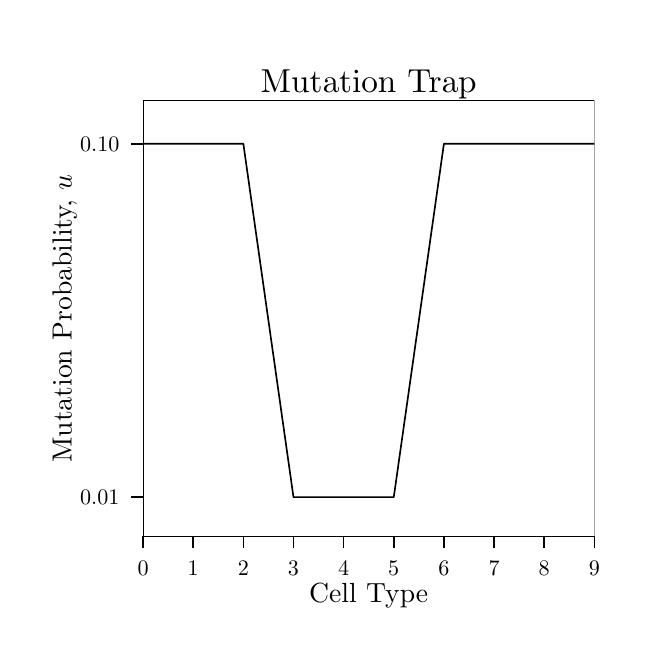
\begin{tikzpicture}[x=1pt,y=1pt]
\definecolor[named]{fillColor}{rgb}{1.00,1.00,1.00}
\path[use as bounding box,fill=fillColor,fill opacity=0.00] (0,0) rectangle (216.81,216.81);
\begin{scope}
\path[clip] (  0.00,  0.00) rectangle (216.81,216.81);
\definecolor[named]{drawColor}{rgb}{1.00,1.00,1.00}
\definecolor[named]{fillColor}{rgb}{1.00,1.00,1.00}

\path[draw=drawColor,line width= 0.6pt,line join=round,line cap=round,fill=fillColor] ( -0.00,  0.00) rectangle (216.81,216.81);
\end{scope}
\begin{scope}
\path[clip] ( 41.69, 32.98) rectangle (204.76,190.48);
\definecolor[named]{fillColor}{rgb}{1.00,1.00,1.00}

\path[fill=fillColor] ( 41.69, 32.98) rectangle (204.76,190.48);
\definecolor[named]{drawColor}{rgb}{0.00,0.00,0.00}

\path[draw=drawColor,line width= 0.6pt,line join=round] ( 41.69,174.87) --
	( 59.81,174.87) --
	( 77.93,174.87) --
	( 96.05, 47.17) --
	(114.17, 47.17) --
	(132.29, 47.17) --
	(150.41,174.87) --
	(168.53,174.87) --
	(186.65,174.87) --
	(204.76,174.87);

\path[draw=drawColor,line width= 0.6pt,line join=round,line cap=round] ( 41.69, 32.98) rectangle (204.76,190.48);
\end{scope}
\begin{scope}
\path[clip] (  0.00,  0.00) rectangle (216.81,216.81);
\definecolor[named]{drawColor}{rgb}{0.00,0.00,0.00}

\node[text=drawColor,anchor=base east,inner sep=0pt, outer sep=0pt, scale=  0.80] at ( 33.15, 44.41) {0.01};

\node[text=drawColor,anchor=base east,inner sep=0pt, outer sep=0pt, scale=  0.80] at ( 33.15,172.11) {0.10};
\end{scope}
\begin{scope}
\path[clip] (  0.00,  0.00) rectangle (216.81,216.81);
\definecolor[named]{drawColor}{rgb}{0.00,0.00,0.00}

\path[draw=drawColor,line width= 0.6pt,line join=round] ( 37.42, 47.17) --
	( 41.69, 47.17);

\path[draw=drawColor,line width= 0.6pt,line join=round] ( 37.42,174.87) --
	( 41.69,174.87);
\end{scope}
\begin{scope}
\path[clip] (  0.00,  0.00) rectangle (216.81,216.81);
\definecolor[named]{drawColor}{rgb}{0.00,0.00,0.00}

\path[draw=drawColor,line width= 0.6pt,line join=round] ( 41.69, 28.71) --
	( 41.69, 32.98);

\path[draw=drawColor,line width= 0.6pt,line join=round] ( 59.81, 28.71) --
	( 59.81, 32.98);

\path[draw=drawColor,line width= 0.6pt,line join=round] ( 77.93, 28.71) --
	( 77.93, 32.98);

\path[draw=drawColor,line width= 0.6pt,line join=round] ( 96.05, 28.71) --
	( 96.05, 32.98);

\path[draw=drawColor,line width= 0.6pt,line join=round] (114.17, 28.71) --
	(114.17, 32.98);

\path[draw=drawColor,line width= 0.6pt,line join=round] (132.29, 28.71) --
	(132.29, 32.98);

\path[draw=drawColor,line width= 0.6pt,line join=round] (150.41, 28.71) --
	(150.41, 32.98);

\path[draw=drawColor,line width= 0.6pt,line join=round] (168.53, 28.71) --
	(168.53, 32.98);

\path[draw=drawColor,line width= 0.6pt,line join=round] (186.65, 28.71) --
	(186.65, 32.98);

\path[draw=drawColor,line width= 0.6pt,line join=round] (204.76, 28.71) --
	(204.76, 32.98);
\end{scope}
\begin{scope}
\path[clip] (  0.00,  0.00) rectangle (216.81,216.81);
\definecolor[named]{drawColor}{rgb}{0.00,0.00,0.00}

\node[text=drawColor,anchor=base,inner sep=0pt, outer sep=0pt, scale=  0.80] at ( 41.69, 18.93) {0};

\node[text=drawColor,anchor=base,inner sep=0pt, outer sep=0pt, scale=  0.80] at ( 59.81, 18.93) {1};

\node[text=drawColor,anchor=base,inner sep=0pt, outer sep=0pt, scale=  0.80] at ( 77.93, 18.93) {2};

\node[text=drawColor,anchor=base,inner sep=0pt, outer sep=0pt, scale=  0.80] at ( 96.05, 18.93) {3};

\node[text=drawColor,anchor=base,inner sep=0pt, outer sep=0pt, scale=  0.80] at (114.17, 18.93) {4};

\node[text=drawColor,anchor=base,inner sep=0pt, outer sep=0pt, scale=  0.80] at (132.29, 18.93) {5};

\node[text=drawColor,anchor=base,inner sep=0pt, outer sep=0pt, scale=  0.80] at (150.41, 18.93) {6};

\node[text=drawColor,anchor=base,inner sep=0pt, outer sep=0pt, scale=  0.80] at (168.53, 18.93) {7};

\node[text=drawColor,anchor=base,inner sep=0pt, outer sep=0pt, scale=  0.80] at (186.65, 18.93) {8};

\node[text=drawColor,anchor=base,inner sep=0pt, outer sep=0pt, scale=  0.80] at (204.76, 18.93) {9};
\end{scope}
\begin{scope}
\path[clip] (  0.00,  0.00) rectangle (216.81,216.81);
\definecolor[named]{drawColor}{rgb}{0.00,0.00,0.00}

\node[text=drawColor,anchor=base,inner sep=0pt, outer sep=0pt, scale=  1.00] at (123.23,  9.03) {Cell Type};
\end{scope}
\begin{scope}
\path[clip] (  0.00,  0.00) rectangle (216.81,216.81);
\definecolor[named]{drawColor}{rgb}{0.00,0.00,0.00}

\node[text=drawColor,rotate= 90.00,anchor=base,inner sep=0pt, outer sep=0pt, scale=  1.00] at ( 15.92,111.73) {Mutation Probability, $u$};
\end{scope}
\begin{scope}
\path[clip] (  0.00,  0.00) rectangle (216.81,216.81);
\definecolor[named]{drawColor}{rgb}{0.00,0.00,0.00}

\node[text=drawColor,anchor=base,inner sep=0pt, outer sep=0pt, scale=  1.20] at (123.23,193.49) {Mutation Trap};
\end{scope}
\end{tikzpicture}
